\subsection{Running Games}
ScriptButler offers game designers the ability to run their game in a browser. In the original implementation, this feature is coupled with the editor. However, we separate it and extend its capabilities to provide playtesting support using a \emph{salix} web app. At its heart, the salix web app provides game designers the ability to run their game and to see it graphically represented through a Web GUI. We use the Web GUI because Rascal does not possess the feature to represent the game graphically or to 'wait' for user input. We leverage this weakness as a strength by also extending the Web GUI with useful playtesting tools. 

The GUI provides a list of victory conditions and whether or not they are true in the current level state. Game designers can use this feature to check their assumptions of what their victory conditions are. They can create a level state where they think certain conditions should be true and then check whether or not they actually are. The GUI also provides a list of rules, how many times they were used in the last turn and what they look like when compiled. The last part is probably more useful to engine developers, which is why it's hidden from sight by default. Game designers can use this feature to check whether the rules actually run when they intend them to, and how many times they match. Finally, the GUI provides game designers with a \emph{'layered'} view of their level. A 'layered' view is a representation of the level where objects are separated based on which collision layer they appear on. This feature provides an easy way for users to see all objects on a particular pixel that may otherwise be hidden by objects they are stacked under.

The Web GUI provides tool to support the game designers when they debug their games. It uses salix which means it is, for a majority, written in Rascal. This design decision makes it easier to edit for those seeking to modify or extend the tool. The downside to our approach is that salix is still a relatively new library and suffers in regard to response times. Figure \ref{fig:salix_webserver} shows an example of Web GUI's appearance. 

\begin{figure}[!t]
    \centering
    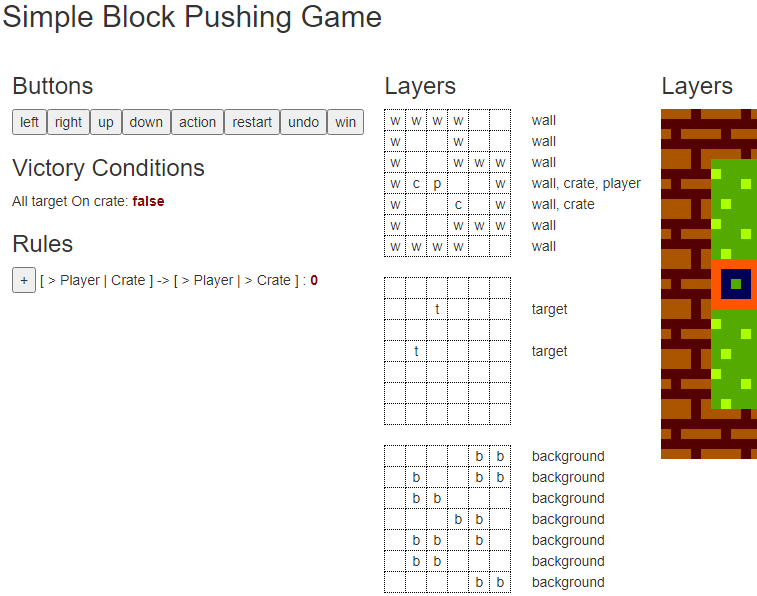
\includegraphics[width=1\textwidth]{images/Rascal Salix.png}
    \caption{Salix web app}
    \label{fig:salix_webserver}
\end{figure}